% Chapter Template

\chapter{Nuclear Shell Model} % Main chapter title

\label{Chapter 2} % Change X to a consecutive number; for referencing this chapter elsewhere, use \ref{ChapterX}

\lhead{Chapter 2. \emph{Nuclear Shell Model}} % Change X to a consecutive number; this is for the header on each page - perhaps a shortened title

\section{Introduction}

The nuclear shell model is one way to model a nucleus. It is analogous to the atomic shell model. In the atomic shell model, the electrons of an atom move in the central Coulomb potential created by its nucleus. The discrete states, or shells, created by solving the Schr\"odinger equation with the Coulomb potential are filled up in order of energy by electrons, obeying the Pauli principle. There are discontinuities in the properties of atoms at shell closures\cite{atomicshell}.

In a nucleus, this approach explains observed phenomena. There are discontinuities of nuclear properties at the so called \textit{magic numbers} of nucleons\cite{mayer}. These numbers are $2, 8, 20, 28, 50, 82, \mathrm{and }126$\cite{krane}. This can be explained by shell structure, but not by collective models of the nucleus.

The difference between the atomic and nuclear shell models is that in the atom, the electrons move in an external potential, rather than one created by the nucleons themselves. This is a potential problem. Short-range interactions distort the picture of nucleons moving independently in a shell structure.

However, the shell model is still useful, especially when considering single nucleon transfer. This is because of its focus on the motion of individual particles. Also, single nuclear transfer reaction cross-sections depend on the matrix element of the initial and final states. This is essentially how much the final nucleus looks like a core with a single excited neutron outside of it, i.e. a shell model state. In stable nuclei, the shell gaps still hold even far away from magic numbers. This means that for excited states of stable nuclei away from shell closures, the low-lying excitations do not contain large contributions from shell model states from different major shells. The shell model also performs well near to the magic numbers\cite{shellmodelmagic}.

\subsection{The Nuclear Hamiltonian}

The nucleus is a many-body problem. The force that holds the nucleus together is the nuclear force. This force cannot be easily described. Including only two-body interactions between nucleons, the nuclear Hamiltonian looks like

\begin{equation}
\hat{H} = \sum_{i=1}^{A} \frac{{\bf \hat{p}}_i^2}{2m_i} + \sum_{i>k=1}^{A} \hat{V}({\bf r}_i-{\bf r}_k)\mathrm{,}
\end{equation}

in a system of $A$ nucleons, ${\bf p}_i$, $m_i$ are the momentum and mass of the $i$th nucleon, and  $\hat{V}({\bf r}_i-{\bf r}_k)$ is the potential between two nucleons at positions ${\bf r}_i$ and ${\bf r}_k$.

This Hamiltonian includes a kinetic energy term for each nucleon, and then an interaction potential between each pair of nucleons. Solving the Schr{\"o}dinger equation for this Hamiltonian becomes computationally very intensive at increasing $A$, so only very light nuclei have been solved this way\cite{latticeqcd}. Even this does not account for three-body interactions.

There are too many nucleons in a nuclei to solve exactly, and not enough to treat statistically. Therefore, models and approximations must be utilised to make accurate predictions about nuclear structure. One way of doing this is to write the Hamiltonian as

\begin{equation}
\hat{H} =  \sum_{i=1}^{A} \bigg [ \frac{{\bf \hat{p}}_i^2}{2m_i} + U_i({\bf r}) \bigg ] + \sum_{i>k=1}^{A} \hat{V}({\bf r}_i-{\bf r}_k) -  \sum_{i=1}^{A}  U_i({\bf r}) \mathrm{,}
\end{equation}

where $U_i$ is a central one-body \textit{mean-field} potential. The two-body potential minus the mean-field potential is the \textit{residual interaction}. $U_i$ is chosen such that the effect of the residual interactions is minimised.


\subsection{Nuclear Potentials} 

The mean-field potential must be chosen to minimise the residual interactions. One way of doing this is by calculating a self-consistent Schr\"odinger equation. This is done by making an initial guess of $U_i({\bf r})$ and   solving the Schr\"odinger equation. The wavefunctions $\psi_i$ generated by this are then inserted back into the Schr\"odinger equation to solve for an improved $U_i({\bf r})$. This continues until $U_i({\bf r})$ and $\psi_i$ converge. This method is the Hartree-Fock Method\cite{hartreefock}.

This is both computationally expensive and sensitive to the initial conditions. An alternative to this is to choose a sensible form of potential, then fit the parameters to experiment.

A sensible first choice of potential is the simple harmonic oscillator,

\begin{equation}
V(r) = \frac{1}{2}m \omega^2 r^2\mathrm{,}
\end{equation}

where $m$ is the mass of the nucleon and $\omega$ is the angular frequency of oscillation. The advantage of this model is that it has an exact solution. It also predicts the magic numbers $N = 2,~8,~20$, but fails at larger energies. This makes sense, because as $r \to \infty, V \to \infty$ in the harmonic oscillator. In reality, the potential must be zero at large distances because of the short range of the nuclear force. 

A potential which is often chosen is the Woods-Saxon potential\cite{woodssaxon}

\begin{equation}
V(r) = - \frac{V_0}{1 + \exp [(r - R)/a ]}\mathrm{,}
\end{equation}

where $V_0$ is the depth of the potential, $a$ is the diffuseness parameter, and $R$ is the nuclear radius. This function replicates the charge and matter densities of the nucleus. This again reproduces the first three magic numbers, but fails after that. 

The answer to the problem of the wrong magic numbers is to introduce a spin-orbit term to the potential\cite{mayer,jensen}. This is a property  of the strong interaction. Unlike in atomic physics, the nuclear spin orbit interaction decreases the energy of aligned orbital and spin angular momentum, and vice-versa. The form of the spin-orbit term is

\begin{equation}
V_{SO}(r) = -V_{\ell s}\frac{1}{r}\frac{\partial V(r)}{\partial r} \boldsymbol{\hat{\ell}} {\bf \cdot} {\bf \hat{s}} \mathrm{,}
\end{equation}

where $\boldsymbol{\hat{\ell}}$ and ${\bf \hat{s}}$ are the orbital and spin angular momentum operators, and $V_{\ell s}$ is a constant which can be fit empirically.

Overall, the difference in the energy ordering of states in the three models is shown in Figure~\ref{shellModels}. The magic numbers predicted by the Woods-Saxon with spin-orbit potential replicate the observed magic numbers.

\begin{figure}[h]	
\vspace*{-2cm}
    \makebox[\linewidth]{
        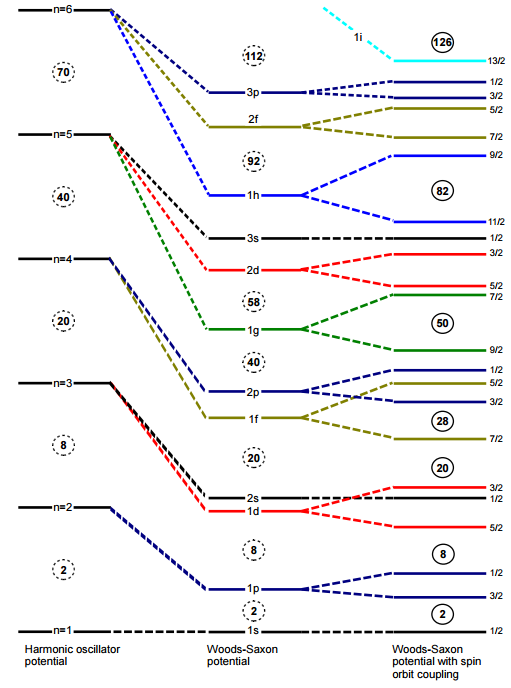
\includegraphics[width=1.3\linewidth]{shellmodelcomparison}	
		}
			\caption[Comparison of the harmonic oscillator, Woods-Saxon, and Woods-Saxon with spin orbit potentials for use in the shell model]{A comparison of shell models built with the harmonic oscillator potential (left), the Woods-Saxon potential (centre), and the Woods-Saxon with spin orbit term (right)\cite{sharp}.}
		\label{shellModels}
\end{figure}
\FloatBarrier


The amount of energy splitting the spin-orbit interaction causes between parallel spin-orbit states and antiparallel spin-orbit states can be easily shown. The expectation value of ${\boldsymbol{\hat{\ell}}} {\bf \cdot} {\bf \hat{s}}$ is

\begin{equation}
\langle {\boldsymbol{\hat{\ell}}} {\bf \cdot} {\bf \hat{s}} \rangle = \frac{\hbar^2}{2} \bigg [ j(j+1) - l(l+1) -s(s+1) \bigg ].
\end{equation}

Because nucleons are fermions, $s = \frac{1}{2}$, so the energy splitting between two states with the same $\ell$ but with oppositely aligned spins is

\begin{equation}
\langle {\boldsymbol{\hat{\ell}}} {\bf \cdot} {\bf \hat{s}} \rangle_{j = \ell + \frac{1}{2}} - \langle {\boldsymbol{\hat{\ell}}} {\bf \cdot} {\bf \hat{s}} \rangle_{j = \ell - \frac{1}{2}} = \frac{1}{2}(2 \ell + 1) \hbar^2.
\end{equation}

\subsection{Residual Interactions}

Unfortunately, the shell model is limited, because residual interactions are nearly always significant. To solve for the energies of nuclear states taking residual interactions into account, the residual interactions can be treated as a pertubation to the independent particle Hamiltonian. What is observed in real nuclei are more complicated states which are mixtures of single-particle configurations. The independent particle model wavefunctions $\Phi_j$ make up a basis set, 

\begin{equation}
 | \Psi_i \rangle = \sum_{j} a_{ij} \Phi_j\mathrm{,}
\end{equation}

where $\Psi_i$ is a wavefunction of a real nuclear state and $a_{ij}$ are the amplitudes of each single-particle constituent in $\Psi_i$.
